\begin{center}
    \textbf{Алгебра}
\end{center} 


\samerowans{\begin{problem}{1 (2 балла)}
Найдите значение выражения 
$ \dfrac{11a^6b^3 - (3a^2b)^3}{4a^6b^6} $ при $b=2$.
Сравните его со значением выражения:
$ \dfrac{12^3 \cdot 5^6}{15^4 \cdot 10^4} $
В ответ запишите меньшее из них (только число).
\end{problem}}

\smallskip

\samerowans{\begin{problem}{2а (2 балла)}
Решите уравнение: $\dfrac{5}{6} + \dfrac{4x+6}{5} - 4 = \dfrac{-3x-2}{4}$
\end{problem}}

\smallskip

\samerowans{\begin{problem}{2б (2 балла)}
Решите уравнение: 
\smallskip
$(y - 4)(y + 2) - (y - 2)^2 = 0$
\end{problem}}

\smallskip

\begin{problem}{2в (2 балла)}
Решите уравнение: $\bigl|\,4 - |x-5|\,\bigr|-1=3$
\end{problem}

\smallskip

\noindent\grid{34}{12}

\smallskip

\begin{problem}{3}
Разложите на неразложимые множители:
\end{problem}

\bigskip

\noindent \textbf{3а (2 балла).} $2a^3x^3 - 2a^3x^2 - 10a^2x$

\smallskip

\rowans{1ex}

\bigskip

\noindent \textbf{3б (2 балла).} $x^2 - 3x - 3y - y^2$

\smallskip

\rowans{1ex}

\bigskip

\noindent \textbf{3в (2 балла).} $a^3 + 8b^3 + a^2 - 2ab + 4b^2$

\smallskip

\rowans{1ex}

\smallskip

\samerowans{\begin{problem}{4 (3 балла)}
Лодка за 4 часа по течению и 3 часа против течения проходит 150 км. За 5 часов против течения она проходит на 30 км больше, чем за 2 часа по течению. Найдите скорость лодки по течению.
\end{problem}}

\bigskip

\begin{problem}{5}
График линейной функции проходит через точку $A(-2; 8)$ параллельно прямой $y +2x  = 4$.

\smallskip

\noindent \textbf{5а (1 балл).}~Задайте линейную функцию формулой и постройте её график.

\smallskip

\noindent \textbf{5б (2 балла).	}~Найдите точки на этой прямой, у которых ордината в 2 раза больше абсциссы.
\end{problem}

\smallskip

\noindent\grid{34}{18}

\begin{center}
\textbf{Геометрия}
\end{center}

\samerowans{\begin{problem}{6 (2 балла)}
На прямой отмечены точки $A$, $B$ и $C$ в произвольном порядке. Найдите длину отрезка $MK$, где $M$ --- середина отрезка $AB$, $K$ --- середина $BC$, причем $AB=50$ см, $BC=16$ см.
\end{problem}}

\smallskip

\samerowans{\begin{problem}{7 (2 балла)}
По данным рисунка найдите $\angle ABK$, если $AB \| KN$, $KB$ --- биссектриса $\angle MKN$, $\angle MAB = 78^\circ$.
\end{problem}}

\smallskip

\noindent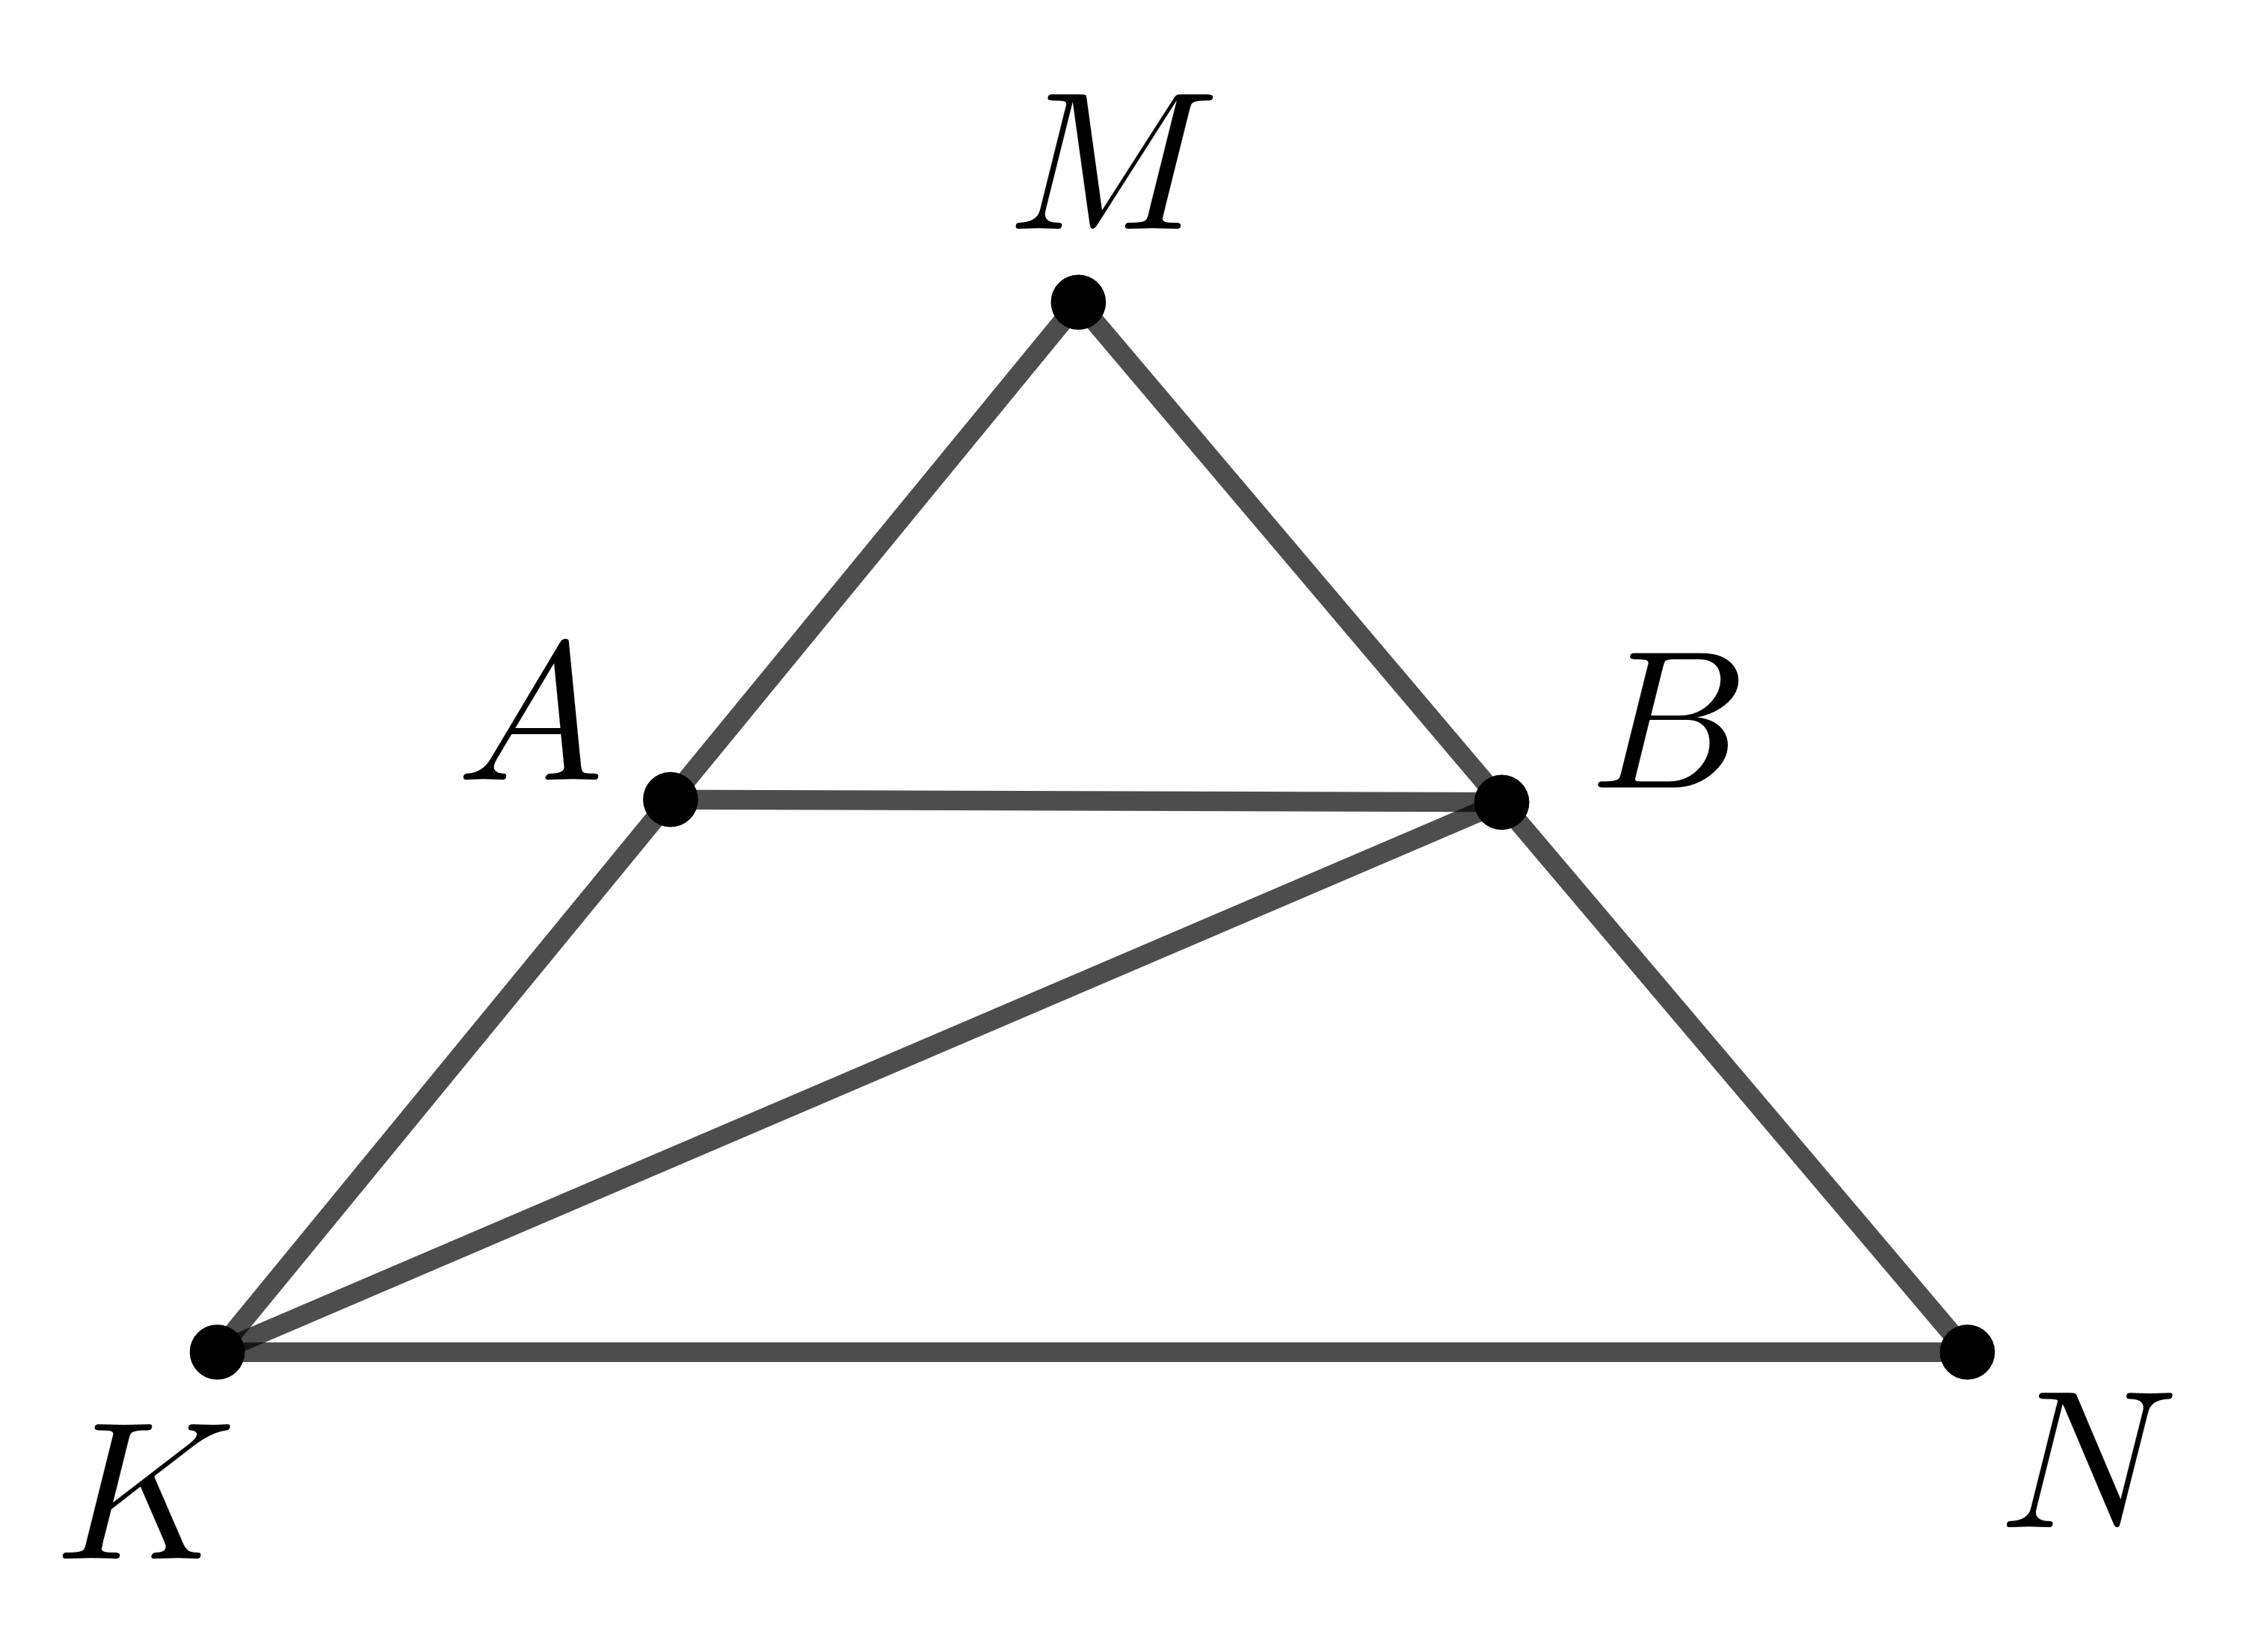
\includegraphics[width=.3\textwidth]{20260404/pics/20260404_inzh_7_v1.png}

\smallskip

\samerowans{\begin{problem}{8 (2 балла)}
В треугольнике $ABC$ стороны $AB$ и $AC$ равны. На стороне $AC$ взяли точки $X$ и $Y$ так, что точка $X$ лежит между точками $A$ и $Y$ и $AX = BX = BY$. Найдите $\angle CBY$, если $\angle CAB = 40^\circ$.
\end{problem}}

\smallskip

\begin{problem}{9 (3 балла)}
В треугольнике $ABC$ $\angle B = 90^\circ$, $BD$ --- высота, $AB = 2BD$. Докажите, что $3AC = 4AD$.
\end{problem}

\noindent\grid{34}{18}

\smallskip

\begin{problem}{10 (4 балла)}
На рисунке $\angle ACD = \angle BCE = 90^\circ$. Сравните периметры треугольников $ADE$ и $ABE$.
\end{problem}
\smallskip

\noindent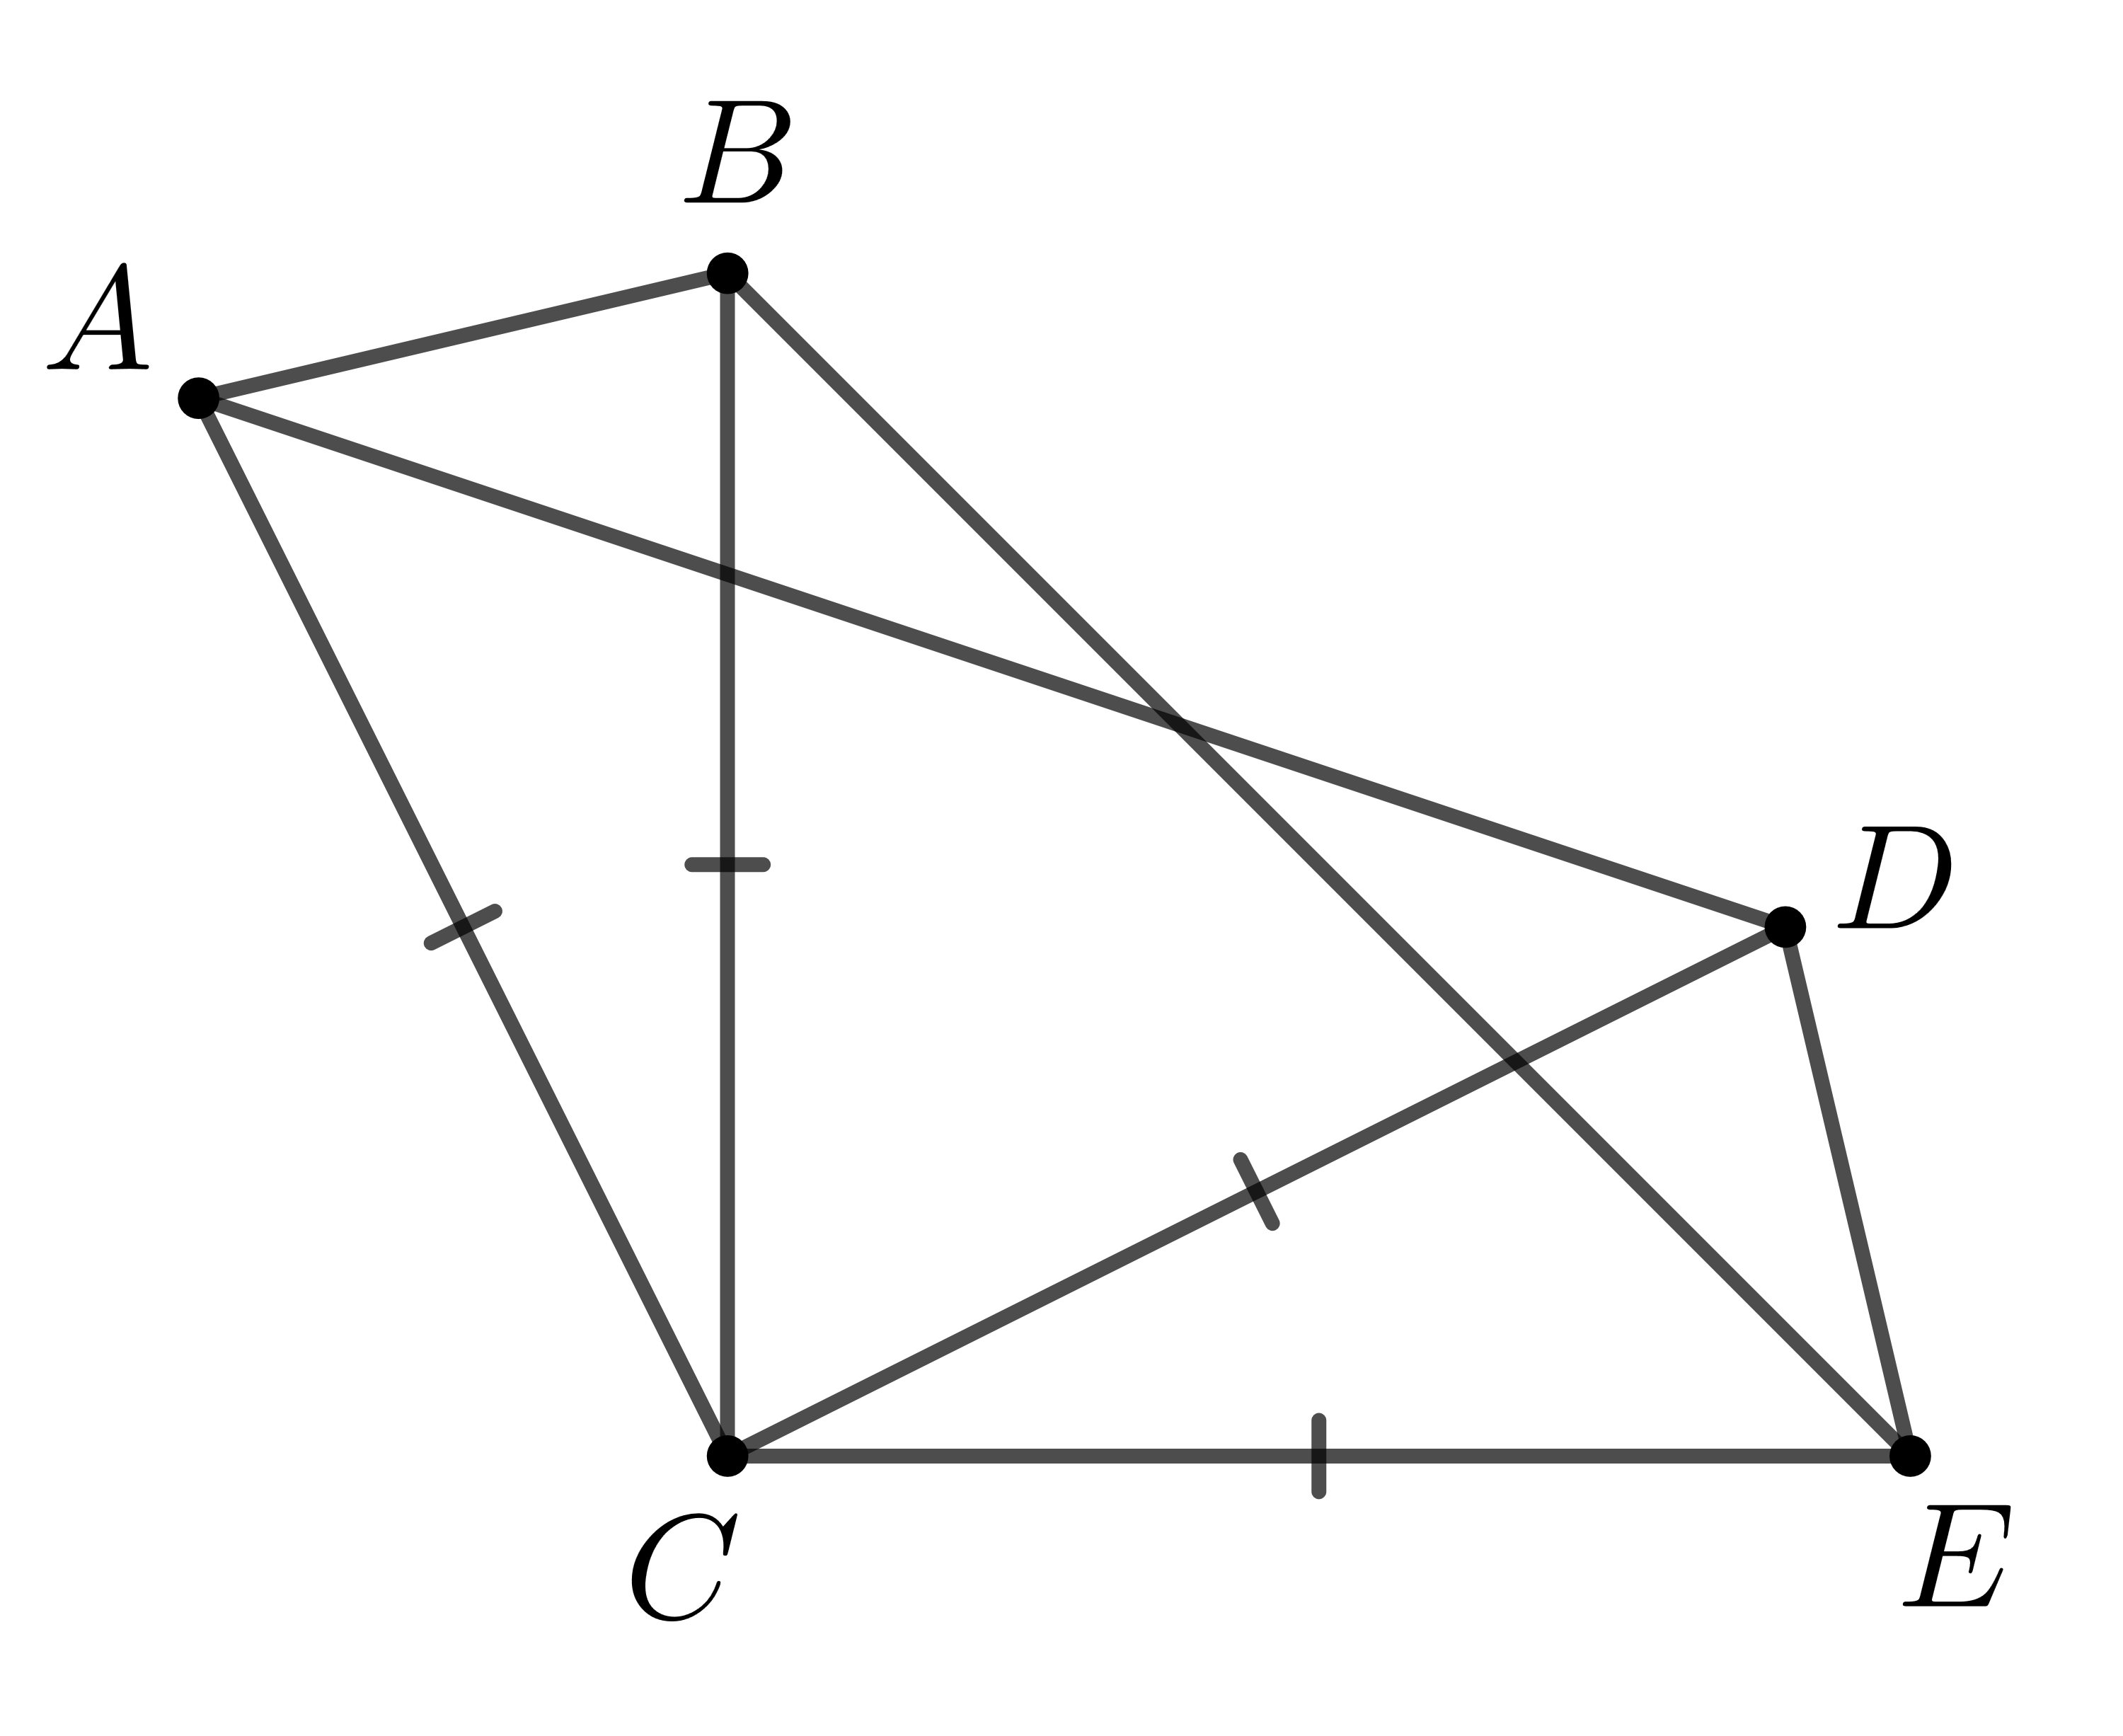
\includegraphics[width=.3\textwidth]{20260404/pics/20260404_inzh_10_v1.png}

\smallskip
\noindent\grid{34}{18}
\smallskip

\begin{center}
\textbf{Дополнительная задача}
\end{center}

\begin{problem}{11 (3 балла)}
Решите ОДНО из заданий по выбору. \\
а) Докажите равенство двух треугольников по стороне, прилежащему к ней углу и высоте, проведённой к этой стороне. \\
б) Найдите значение выражения: $$(a + c)(a - c) - b(2a - b) - (a - b + c)(a - b - c)$$ \\
в) Смешали 30\%-ный раствор соляной кислоты с 10\%-ным раствором, получили 600 г 15\%-ного раствора кислоты. Сколько граммов каждого раствора было взято?
\end{problem}

\smallskip

\noindent\grid{34}{18}